\providecommand{\main}{../main}
\documentclass[../main/main.tex]{subfiles}



\begin{document}

\section{Results and discussion}

We move now to the results obtained from the previously discussed implementation of the TTN structure and learning algorithm. So, in this part, in Subsection \textbf{\ref{ssec:results_comparison}} we begin with a rapid comparison between the performances of a ``pure'' TTN model, previously defined, with a more advanced one with regularisation and batch normalisation techniques. After this point, in Subsection \textbf{\ref{ssec:results_characterisation}} we go on with the characterisation of the advanced structure, in particular with a timing and performance analysis depending on the bond dimension \( \chi \), map type and map order \( d \). To conclude, in Subsection \textbf{\ref{ssec:results_final}} we treat in detail the analysis of the results for the most successful architecture of the TTN trained for this work.

Last but not least, we remark that due to the dimension of the dataset and to the type of computational task, the computational load of the problem is faced using the resources of CloudVeneto computing infrastructure \cite{cloudveneto}. In particular, the following results are obtained using a Virtual Machine (VM) with 15 virtual cores, \( 90 \ \si{GB} \) of RAM and with an NVIDIA Tesla T4 Graphic Processor Unit for TTN training.



\subsection{Comparison between ``pure'' and advanced TTN models}
\label{ssec:results_comparison}

The first study performed is a comparison between the a ``pure'' TTN model, namely a model without regularisation, batch normalisation and activation functions in the inner layers, and a model in which some of the most common Machine Learning techniques are included. In particular, we describe more in detail the additions:
\begin{itemize}
    \item after each layer the Exponential Linear Unit activation function is applied to the output data;
    \item the \( \ell_{2} \) regularisation is imposed to the weights of the tensor nodes;
    \item batch normalisation is employed after each tensor layer.
\end{itemize}


The dataset is preprocessed using an order 2 spherical map, which corresponds 
to having each input features represented by a spin; the models on the other hand are built using a bond dimension of 10 and with a 2-feature contraction architecture.

In order to understand the behaviour of the two aforementioned models, these are trained on a smaller training set of \( n_{\mathrm{train}} = 10^{6} \) samples. Concerning their performances, these are quantified by the metrics of accuracy and loss, which are monitored over the epochs on both training and validation sets, with the ladder composed of \( n_{\mathrm{val}} = 5 \cdot 10^{5} \) samples. The comparison for the loss metric is showed in \figref{fig:results_comparison_loss}, while for the accuracy metric it is showed in \figref{fig:results_comparison_accuracy}.

\begin{figure*}[!h]
    \begin{minipage}[c]{0.50\linewidth}
        \vspace{0pt}
        \centering
        \subfloat[Loss metric over training epochs]{
            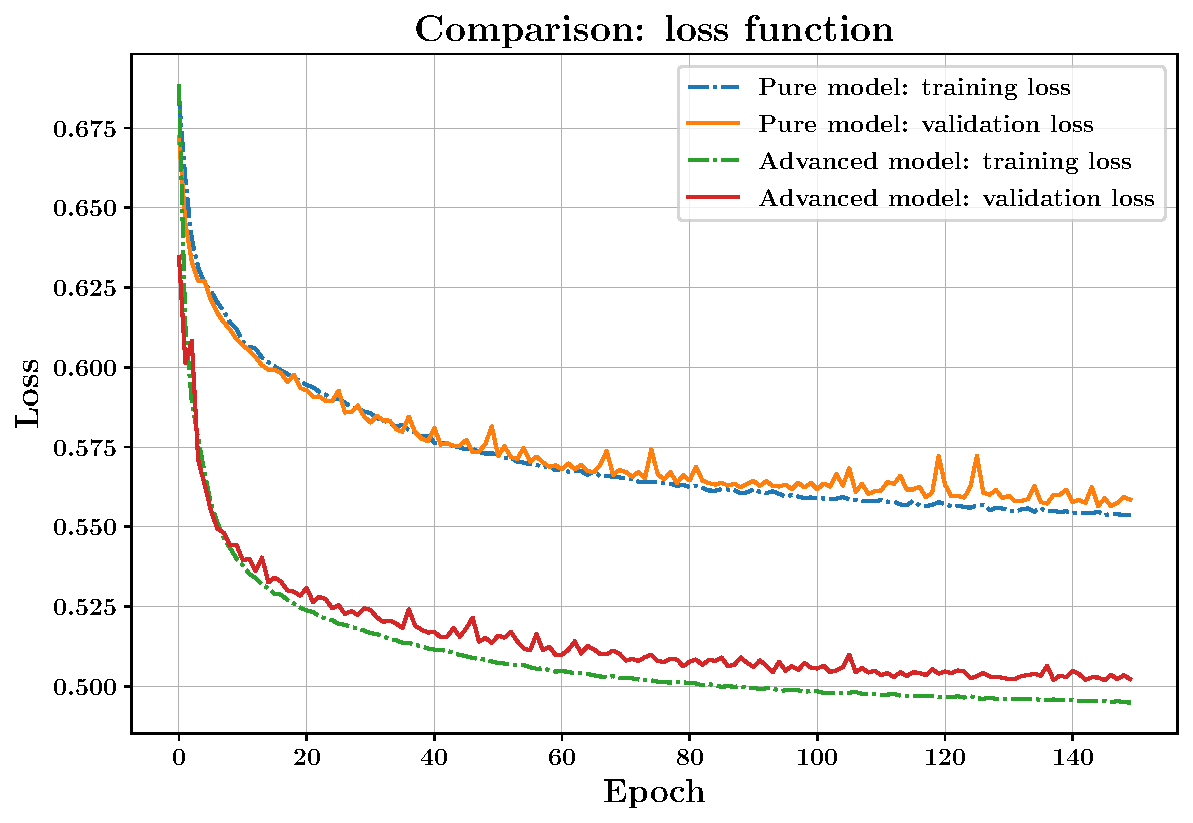
\includegraphics[height=5.8cm]{images/results/comparison/results_comparison_loss.pdf}
            \label{fig:results_comparison_loss}
        }
    \end{minipage}%
    \begin{minipage}[c]{0.50\linewidth}
        \vspace{0pt}
        \centering
        \subfloat[Accuracy metric over training epochs]{
            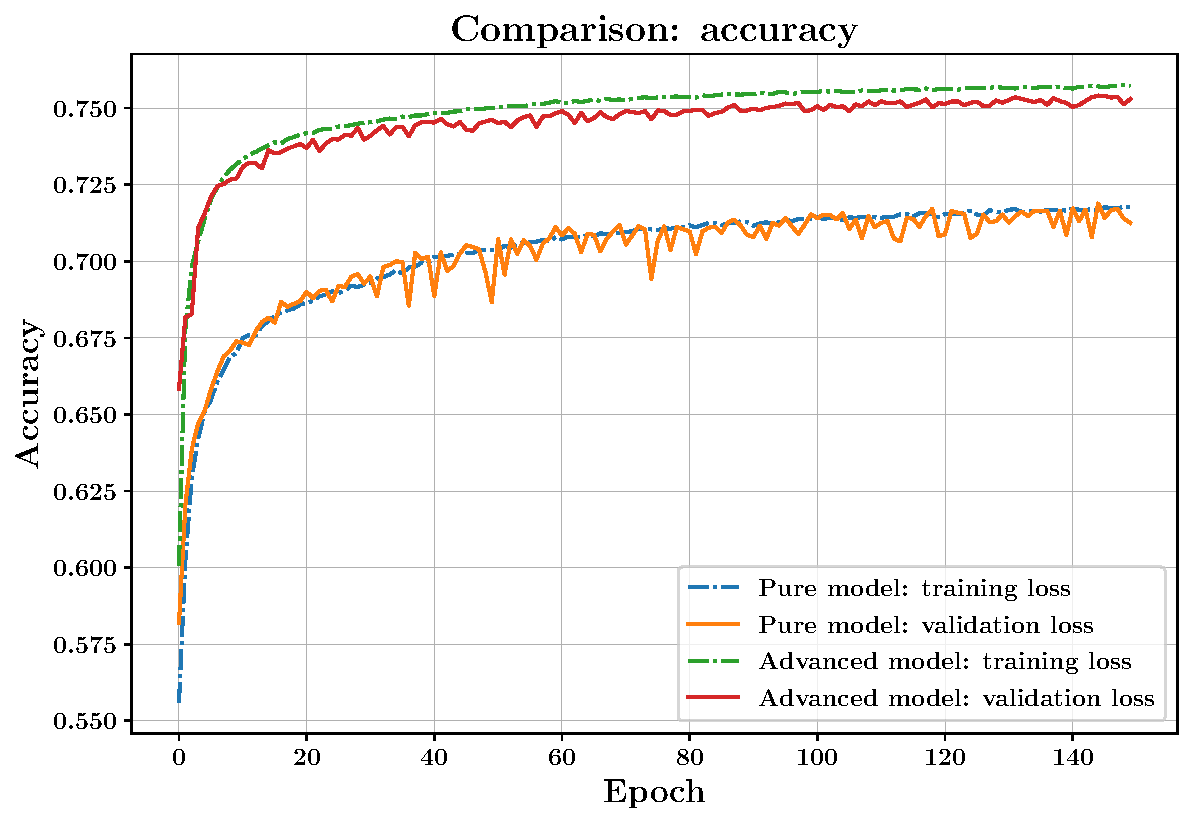
\includegraphics[height=5.8cm]{images/results/comparison/results_comparison_accuracy.pdf}
            \label{fig:results_comparison_accuracy}
        }
    \end{minipage}%
    \caption{Comparison between the ``pure'' TTN model and the advanced one. The trend of the cost function and of the accuracy score during the training are showed in \textbf{\ref{fig:results_comparison_loss}} and \textbf{\ref{fig:results_comparison_accuracy}}, respectively.}
    \label{fig:results_comparison}
\end{figure*}

It is possible to observe how both the models, after the training procedure, have learned to discern signal from background in a way not exactly accurate, but significant. In particular, the advanced model performances overcome the performances of the more simple ``pure'' TTN model on both the training and validation sets. Another thing to remark is the higher stability of the advanced model, visible in the less pronounced fluctuations in the metrics. This fact is of paramount importance when performing hyperparameters tuning, as it leads to more stable and reliable results.



\subsection{Characterisation of advanced TTN model}
\label{ssec:results_characterisation}

Let us focus now on the advanced TTN structure. During the whole learning procedure, from the preprocessing of the input dataset up to the training itself, many hyperparameters have to be chosen. Each of them has a certain impact on the final performance the TTN classifier. Therefore, it is of particular interest to further study the procedure in this sense, characterising the TTN by varying some of its crucial features:
\begin{itemize}
    \item \textbf{bond dimension \( \boldsymbol{\chi} \)}, which establishes the complexity of the model;
    \item \textbf{feature map}, including its type and the order \( d \), offering the possibility to enhance the capability of the model to recognise specific non-linear combinations of the input features;
    \item \textbf{batch size}, which can enhance the parallelisation of the computational task.
\end{itemize}


\paragraph{Bond dimension \( \boldsymbol{\chi} \)}
Let us begin from the most important parameter, namely the bond dimension \( \chi \). The ladder plays a pivotal role in the definition of the architecture since the level of complexity of the model is proportional to its value. In particular a higher bond dimension will result in a higher number of parameters, which may enhance the performance of the network. However, the bond dimension has to be selected carefully since using a too large value enlightens his drawbacks:
\begin{itemize}
    \item the more parameters the model has, the more computationally intensive training and evaluation are;
    \item if the model is too complex for input dataset, it may perform worse than a simpler one due to overfitting.
\end{itemize}
For instance, the number of parameters of the model depending on \( \chi \) is showed in \tabref{tab:results_characterisation_parameters}.


\begin{table}[!h]
    \centering
    \begin{tabular}{cc|cc|cc|cc}
        \toprule
       % \textbf{Bond \newline dimension} & \textbf{Model \\ parameters} &
       % \textbf{Bond \newline dimension} & \textbf{Model \\ parameters} &
       % \textbf{Bond \newline dimension} & \textbf{Model \\ parameters} &
       % \textbf{Bond \newline dimension} & \textbf{Model \\ parameters} \\
        \textbf{Bond} & \textbf{Model} &
        \textbf{Bond} & \textbf{Model} &
        \textbf{Bond} & \textbf{Model} &
        \textbf{Bond} & \textbf{Model} \\
        \textbf{dimension} & \textbf{parameters} &
        \textbf{dimension} & \textbf{parameters} &
        \textbf{dimension} & \textbf{parameters} &
        \textbf{dimension} & \textbf{parameters} \\
        \colrule
        5   & $ \approx 2.73 \cdot 10^{3} $ & 30  & $ \approx 3.84 \cdot 10^{5} $ & 55  & $ \approx 2.34 \cdot 10^{6} $ & 80  & $ \approx 7.18 \cdot 10^{6} $ \\ 
        10  & $ \approx 1.60 \cdot 10^{4} $ & 35  & $ \approx 6.08 \cdot 10^{5} $ & 60  & $ \approx 3.03 \cdot 10^{6} $ & 85  & $ \approx 8.62 \cdot 10^{6} $ \\
        15  & $ \approx 5.03 \cdot 10^{4} $ & 40  & $ \approx 9.05 \cdot 10^{5} $ & 65  & $ \approx 3.86 \cdot 10^{6} $ & 90  & $ \approx 1.02 \cdot 10^{6} $ \\
        20  & $ \approx 1.16 \cdot 10^{5} $ & 45  & $ \approx 1.28 \cdot 10^{6} $ & 70  & $ \approx 4.82 \cdot 10^{6} $ & 95  & $ \approx 1.20 \cdot 10^{7} $ \\ 
        25  & $ \approx 2.24 \cdot 10^{5} $ & 50  & $ \approx 1.76 \cdot 10^{6} $ & 75  & $ \approx 5.92 \cdot 10^{6} $ & 100 & $ \approx 1.40 \cdot 10^{7} $\\  
        \botrule
    \end{tabular}
    \caption{Number of parameters of the TTN depending on \( \chi \), namely the bond dimension of the tensor nodes.}
    \label{tab:results_characterisation_parameters}
\end{table}


In order to study the behaviour of the model depending on \( \chi \), a series of models with different values of \( \chi \) is trained. The best results over training epochs for the metrics of loss, accuracy and AUC are showed in \figref{fig:results_characterisation_bond_metrics}. Concerning the time performances and scaling with \( \chi \), these are visualised in \figref{fig:results_characterisation_bond_timing}.


\begin{figure*}[!h]
    \begin{minipage}[c]{0.333\linewidth}
        \vspace{0pt}
        \centering
        \subfloat[Model lowest loss value]{
            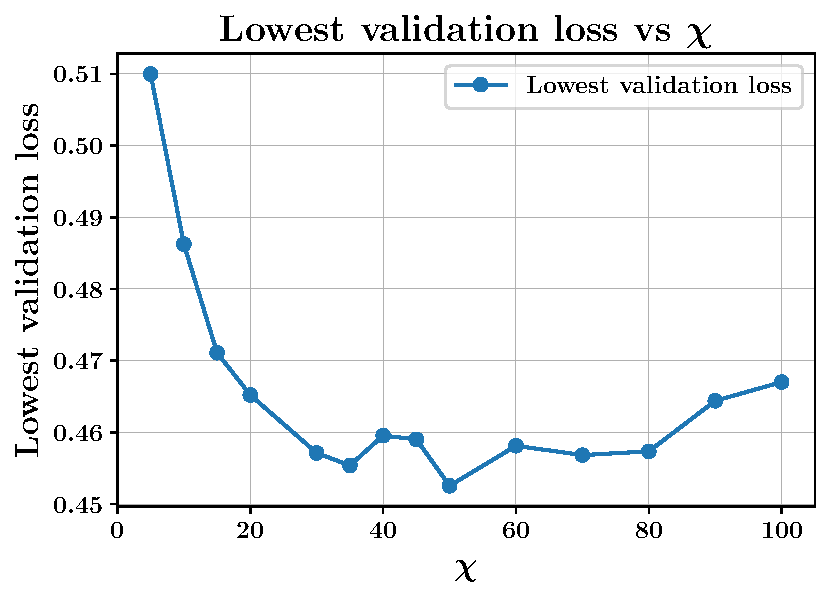
\includegraphics[height=4cm]{images/results/characterisation/results_characterisation_bond_loss.pdf}
            \label{fig:results_characterisation_bond_metrics_loss}
        }
    \end{minipage}%
    \begin{minipage}[c]{0.333\linewidth}
        \vspace{0pt}
        \centering
        \subfloat[Model highest accuracy score]{
            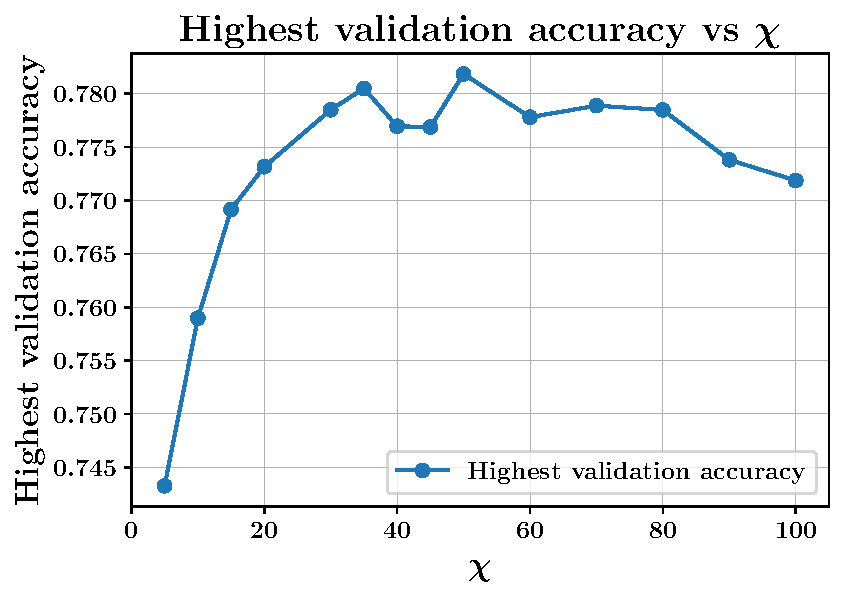
\includegraphics[height=4cm]{images/results/characterisation/results_characterisation_bond_accuracy.pdf}
            \label{fig:results_characterisation_bond_metrics_accuracy}
        }
    \end{minipage}%
    \begin{minipage}[c]{0.333\linewidth}
        \vspace{0pt}
        \centering
        \subfloat[Model highest AUC score]{
            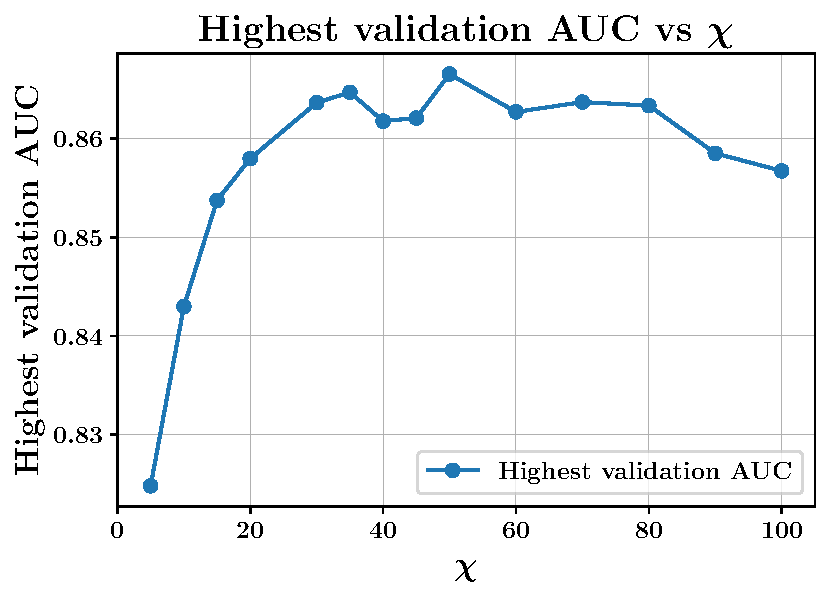
\includegraphics[height=4cm]{images/results/characterisation/results_characterisation_bond_auc.pdf}
            \label{fig:results_characterisation_bond_metrics_auc}
        }
    \end{minipage}%
    \caption{Performance of TTN model depending on the bond dimension. The results are obtained from the validation set, on which the best values over training epochs for the metrics are computed. In particular, in \textbf{\ref{fig:results_characterisation_bond_metrics_loss}} the lowest loss, in \textbf{\ref{fig:results_characterisation_bond_metrics_accuracy}} the highest accuracy and in \textbf{\ref{fig:results_characterisation_bond_metrics_auc}} the highest AUC, depending on the bond dimension \( \chi \).}
    \label{fig:results_characterisation_bond_metrics}
\end{figure*}


\begin{figure*}[!h]
   \begin{minipage}[c]{0.50\textwidth}
        \vspace{0pt}
        \centering
        \subfloat[Model training time per epoch for \( 10^{7} \) samples]{
            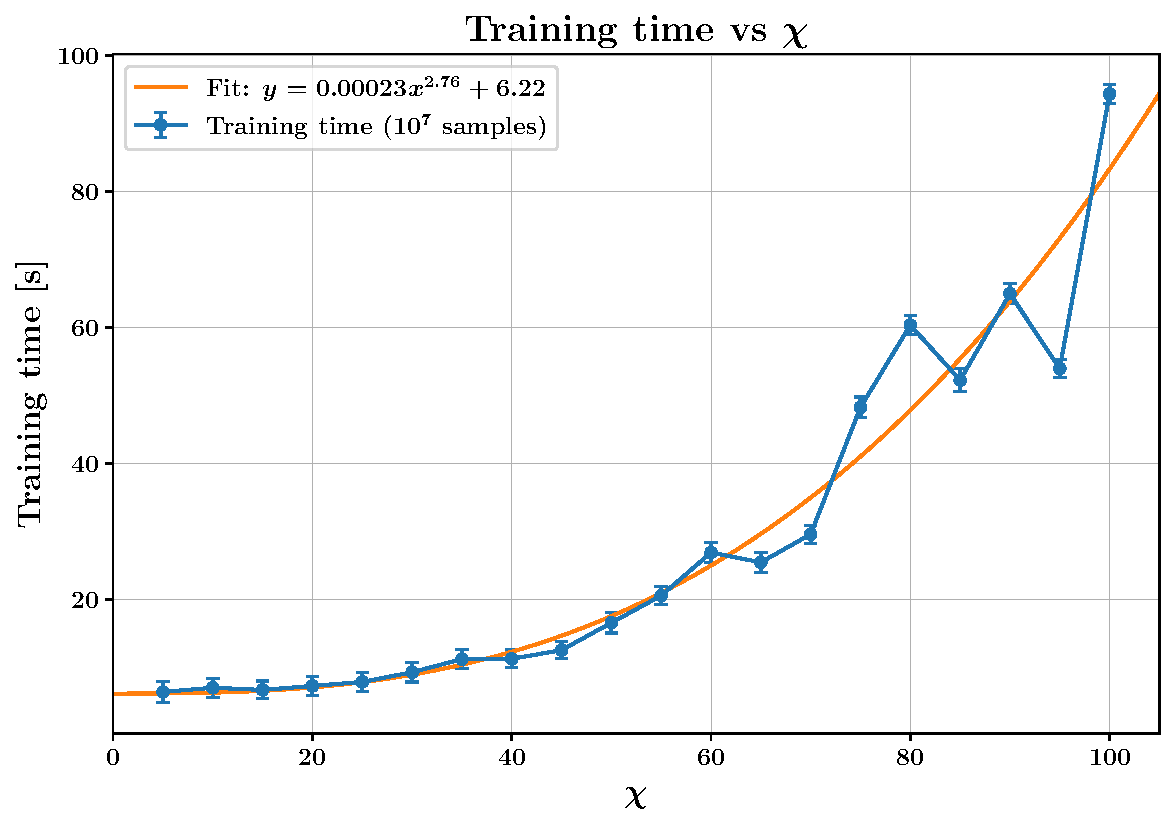
\includegraphics[height=5.8cm]{images/results/characterisation/results_characterisation_bond_training.pdf}
            \label{fig:results_characterisation_bond_timing_training}
        }
    \end{minipage}%
    \begin{minipage}[c]{0.50\textwidth}
        \vspace{0pt}
        \centering
        \subfloat[Model prediction time for \( 5 \cdot 10^{5} \) samples]{
            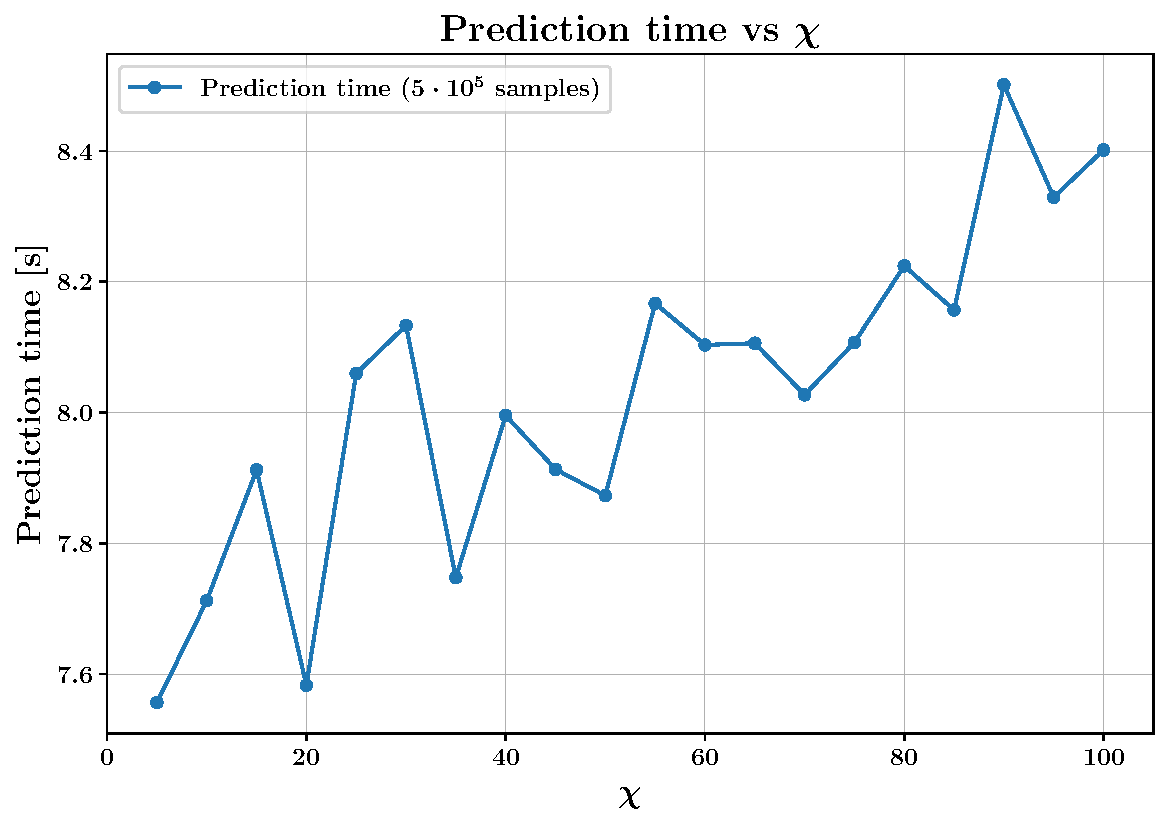
\includegraphics[height=5.8cm]{images/results/characterisation/results_characterisation_bond_prediction.pdf}
            \label{fig:results_characterisation_bond_timing_prediction}
        }
    \end{minipage}%
    \caption{Timing analysis and scaling of TTN classifier depending on the bond dimension \( \chi \). In \figref{fig:results_characterisation_bond_timing_training} the training time per epoch for \( 10^{7} \) samples is showed, while in \figref{fig:results_characterisation_bond_timing_prediction} the prediction time for \( 5\cdot 10^{5} \) samples is visualised.}
    \label{fig:results_characterisation_bond_timing}
\end{figure*}


From the plots of the metrics, it is possible to observe how the performances of the model increase with \( \chi \) up to a value of about \( \chi \approx 50 \), after which the validation accuracy and AUC start to decrease. This behaviour indicates that after that value the model complexity is too high for the input dataset dimension and so it shows overfitting symptoms.

Concerning the timing plots, the training time per epoch for \( 10^{7} \) input samples is showed in \figref{fig:results_characterisation_bond_timing_training}, while the prediction time for \( 5 \cdot 10^{5} \) input samples is showed in \figref{fig:results_characterisation_bond_timing_prediction}. As expected, the training time per epoch increases with \( \chi \). The data points are interpolated using a power law distribution function, namely:
\begin{equation}
    y
    =
    ax^{k} + c
    \quad ,
\end{equation}
obtaining as exponent parameter a value of \( k = 2.76 \). From a theoretical point of view, the expected value is \( k = 3 \), since we are dealing with rank-3 tensors and in the middle layers the tensor nodes have dimension equal to \( \chi^{3} \). On the other hand, the TTN model is trained on a GPU, so the discrepancy can be due to the parallelisation of the computations on the hardware.
Concerning the prediction time for a fixed number of input samples, visualised in \figref{fig:results_characterisation_bond_timing_prediction}, it exhibits a linear trend with higher fluctuations. The ladders can be explained again by the fact that the computations are performed on a GPU, so the overhead time needed for data transfer on the hardware, which is not constant and depends on the system status, has also to be taken into account.


\paragraph{Feature map and map order}
We focus now on the characterisation of the TTN model depending on the feature map applied in the preprocessing and on its order \( d \). The results for this phase are obtained using \( \chi = 35 \), which is the second best result for the bond dimension analysis. We explicitly do not choose the best one with \( \chi = 50 \) due to its computational effort and to time limitations. Moreover, the differences in performances between them are not too significant.

Similarly to what already done for the bond dimension analysis, for the map characterisation the same TTN structure is trained for both spherical and polynomial feature maps and for an order \( d \in \{ 2,3,4,5 \} \).

The results for this study are presented in \tabref{tab:results_characterisation_map}. As it is possible to see, the TTN classifier performances are not significantly affected by the choice of the feature map and by its order. In fact, it is important to remark that the order of the feature map affects only the dimensions and number of parameters in the input layer. This explains the small rise in the training and prediction time for a map of higher order. On the other hand, in terms of absolute performances, it is possible to observe a slight improvement with a rising map order, in particular with a spherical map of order \( d = 5 \).


\begin{table}[!h]
    \centering
    \begin{tabular}{c|@{\extracolsep{0.25cm}} cccc |cccc}
        \toprule
        & \multicolumn{4}{c|}{\textbf{Spherical Map}} &
          \multicolumn{4}{c}{\textbf{Polynomial Map}}\\
          \colrule
        \textbf{Map Order \( \boldsymbol{d} \)}       & 2 & 3 & 4 & 5                & 2 & 3 & 4 & 5 \\
        \colrule
        \textbf{Min loss}       &0.532 & 0.523 & 0.512 & 0.511 & 0.526 & 0.519 & 0.512 & 0.514 \\  
        \textbf{Max accuracy}   &0.777 & 0.781 & 0.781 & 0.782 & 0.781 & 0.781 & 0.781 & 0.781 \\ 
        \textbf{Max AUC}        &0.862 & 0.866 & 0.866 & 0.867 & 0.866 & 0.866 & 0.866 & 0.865 \\  
        \textbf{Training time [s]}   & 120 & 127 & 134 & 140 & 125 & 133 & 141 & 150 \\
        \textbf{Prediction time [s]} & 8.65 & 8.80 & 8.91 & 9.13 & 8.61 & 8.80 & 8.93 & 9.30 \\
        \botrule
    \end{tabular}
    \caption{Results of the feature map and map order characterisation analysis. The training time is obtained for \( 10^{7} \) input samples, while the prediction time for \( 5 \cdot 10^{5} \) input samples.}
    \label{tab:results_characterisation_map}
\end{table}


\paragraph{Batch size}
The last characterisation study involves the hyperparameter of batch size, namely the number of input samples to process before a weight update by the optimiser. This quantity has a crucial role in time needed for the TTN training, as already explained. In fact, a bigger batch size allows to process more samples in parallel, which results in a significant speed enhancement, especially when the training is performed on a GPU. 

Passing to the results, in \figref{fig:results_characterisation_batch} the dependency of the training time on the batch size is visualised. As it is possible to see, smaller values of the batch size translate into very long training times, making the training procedure extremely inefficient and infeasible. Therefore, an optimal choice would be a batch size that can be handled in a single parallel run to maximise the efficiency. In particular, the hardware employed for this work allows a batch size of \( \sim 10^{4} \). For this reason, all the tests with this parameter fixed are done with a minibatch of \( 10^{4} \) samples.

\begin{figure*}[!h]
    \centering
    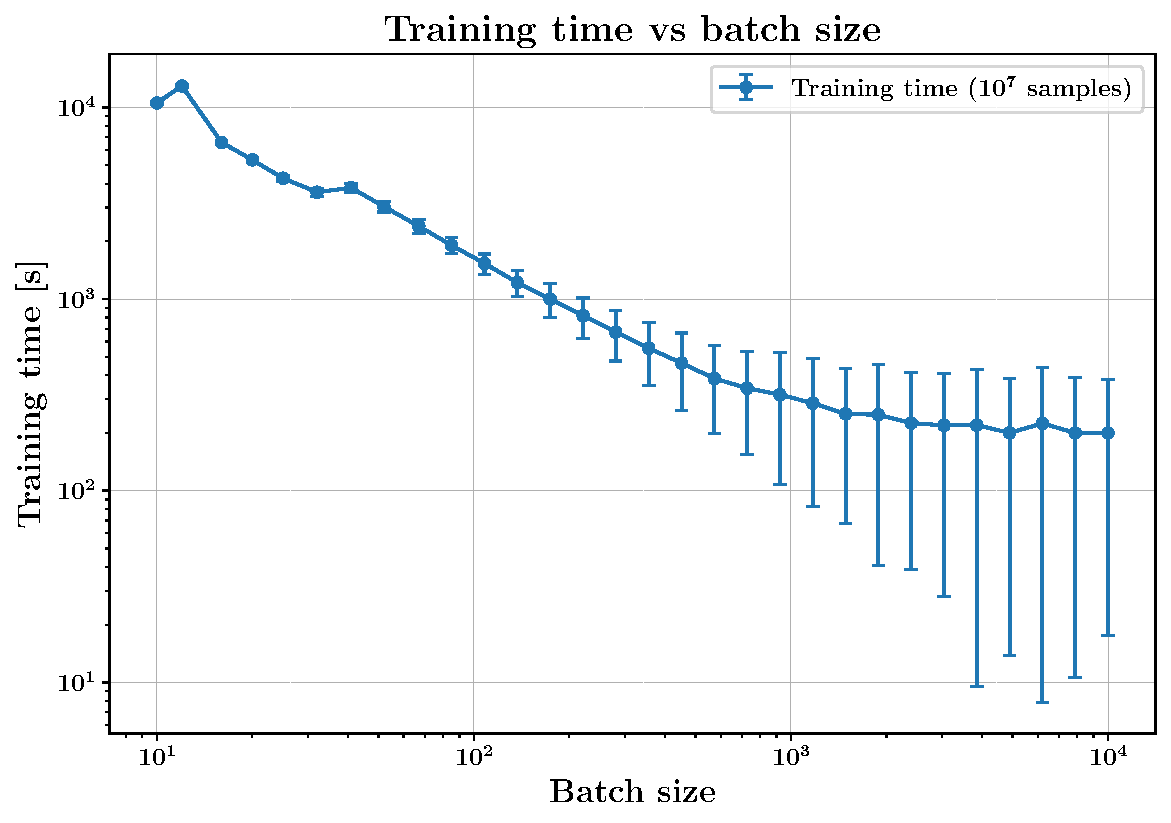
\includegraphics[width=0.5\textwidth]{images/results/characterisation/results_characterisation_batch.pdf}
    \caption{TTN classifier training time per epoch for \( 10^{7} \) input samples depending on the batch size.}
    \label{fig:results_characterisation_batch}
\end{figure*}



\subsection{Final model results}
\label{ssec:results_final}

After having characterised some of the main hyperparameters of the TTN classifier, we combine all the information from the previous analyses to produce the final structure treated. The ladder is trained for a higher number of epochs in order to extract the most promising results of this work. For the sake of completeness, the main parameters used for this last run are given in \tabref{tab:results_final_parameters}. On the other hand, the results obtained for the metrics on training and validation sets are visualised in \figref{fig:results_final_metrics}.


\begin{table}[!h]
    \centering
    \begin{tabular}{cc||cc}
        \toprule
        \multicolumn{2}{c}{\textbf{Feature Map}} &
        \multicolumn{2}{c}{\textbf{Model architecture}} \\
        \colrule
        Type  & \texttt{Spherical}   & \( \chi \)   & 50     \\
        Order    & 5   & Activation    & \texttt{Elu}      \\
        \toprule
        \multicolumn{2}{c}{\textbf{Training Parameters}} &
        \multicolumn{2}{c}{\textbf{Number of samples}}  \\
        \colrule
        Batch size      & $10^4$  & Train set  & $10^7$     \\
        Epochs          & 500   & Validation set   & $5\cdot10^5$      \\
        Optimizer       & \texttt{Adam}   & Test set   & $5\cdot10^5$      \\
        \botrule
    \end{tabular}
    \caption{Hyperparameters for final TTN model, from which the best results obtained in this work are extracted.}
    \label{tab:results_final_parameters}
\end{table}


%\begin{table}[!h]
%    \centering
%    \begin{tabular}{c|cc}
%        \toprule
%        
%        \multirow{2}{*}{\textbf{Feature Map}} &Type   & \texttt{Spherical}  \\
%                                              & Order & 5  \\
%        \colrule
%        \multirow{2}{*}{\textbf{Model architecture}} & Bond dimension   & 50     \\
%                                                     & Activation       & \texttt{Elu}  \\
%        \colrule
%        \multirow{3}{*}{\textbf{Training Parameters}} & Batch size      & $10^4$     \\  
%                                                      & Epochs          & 500          \\
%                                                      & Optimizer       & \texttt{Adam}\\
%        \colrule
%        \multirow{3}{*}{\textbf{Number of samples}}  &  Train set      & $10^7$     \\
%                                                     & Validation set  & $5\cdot10^5$      \\
%                                                     & Test set        & $5\cdot10^5$      \\
%        \botrule
%    \end{tabular}
%    \caption{Results of the test for signal integrity with several types of cable and comparison %between them.}
%    \label{tab:Cable}
%\end{table}
%


\begin{figure*}[h]
    \begin{minipage}[c]{0.333\linewidth}
        \vspace{0pt}
        \centering
        \subfloat[Loss over training epochs]{
            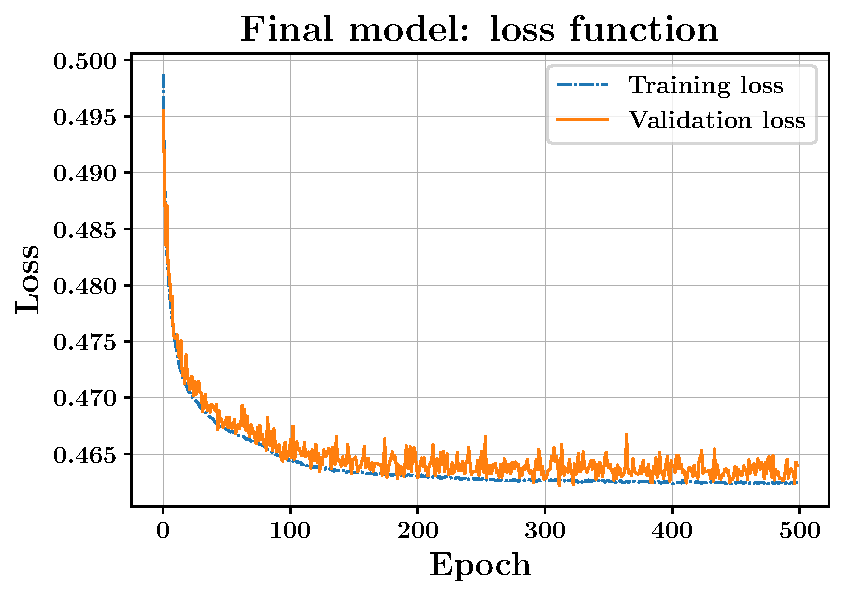
\includegraphics[width=\textwidth]{images/results/final/results_final_loss.pdf}
            \label{fig:results_final_metrics_loss}
        }
    \end{minipage}%
    \begin{minipage}[c]{0.333\linewidth}
        \vspace{0pt}
        \centering
        \subfloat[Accuracy over training epochs]{
            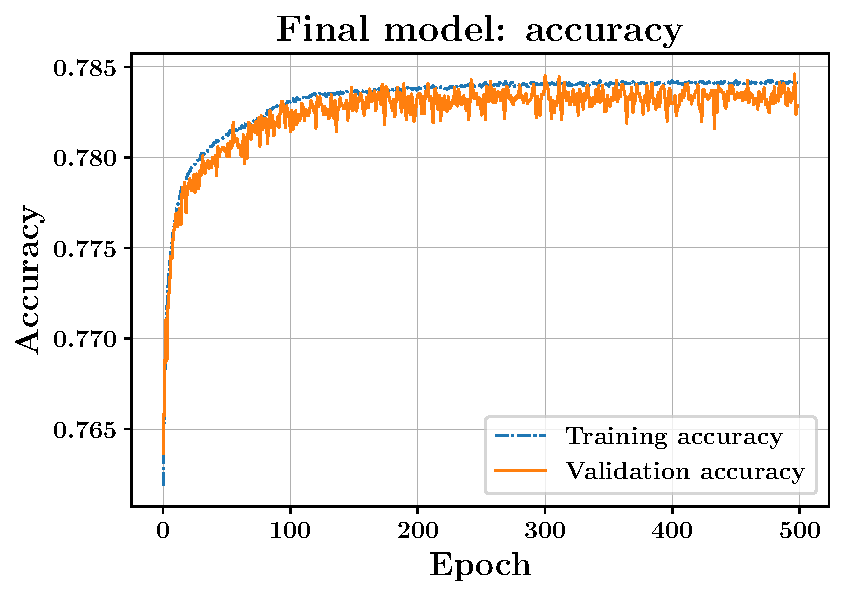
\includegraphics[width=\textwidth]{images/results/final/results_final_accuracy.pdf}
            \label{fig:results_final_metrics_accuracy}
        }
    \end{minipage}%
    \begin{minipage}[c]{0.333\linewidth}
        \vspace{0pt}
        \centering
        \subfloat[AUC over training epochs]{
            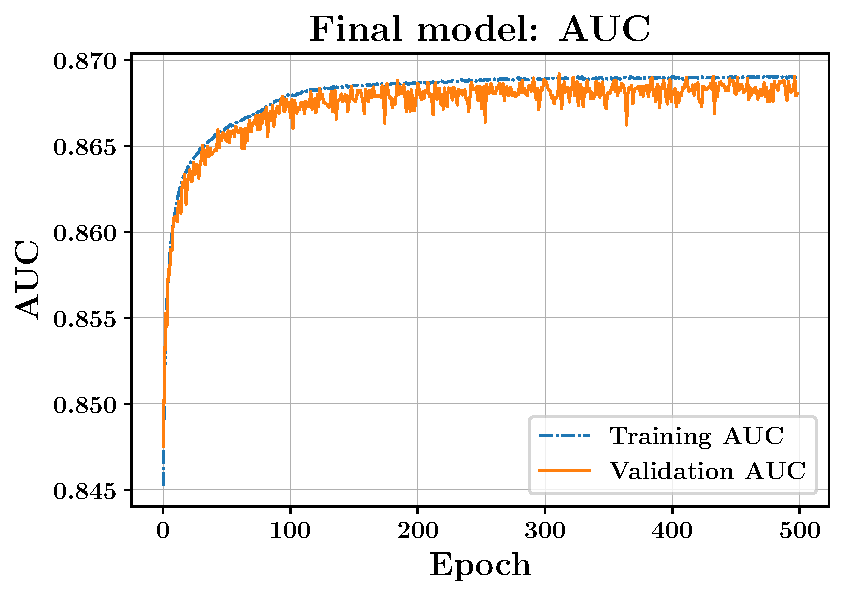
\includegraphics[width=\textwidth]{images/results/final/results_final_auc.pdf}
            \label{fig:results_final_metrics_auc}
        }
    \end{minipage}%
    \caption{Final TTN model metrics computed on training and validation sets over training epochs, with the loss in \textbf{\ref{fig:results_final_metrics_loss}}, the accuracy in \textbf{\ref{fig:results_final_metrics_accuracy}} and the AUC in \textbf{\ref{fig:results_final_metrics_auc}}.}
    \label{fig:results_final_metrics}
\end{figure*}


At the end of the training procedure the best model is saved in a \texttt{hdf5} file format in order retrieve the model with the best validation AUC over the training epochs. In particular, this is possible through a series of ``callbacks'' defined inside TensorFlow framework, so that the model saved is not the one at the last epoch, but the most performing one. In order to quantify the goodness of this model, we extract from it its ROC curve and ``confusion matrix'' calculated on a test set of \( 5 \cdot 10^{5} \) samples. Then, the ladders are visualised in \figref{fig:results_final_roc} and \figref{fig:results_final_cf}, respectively.


\begin{figure*}[!h]
    \begin{minipage}[c]{0.49\linewidth}
        \vspace{0pt}
        \centering
        \subfloat[Final model ROC curve]{
            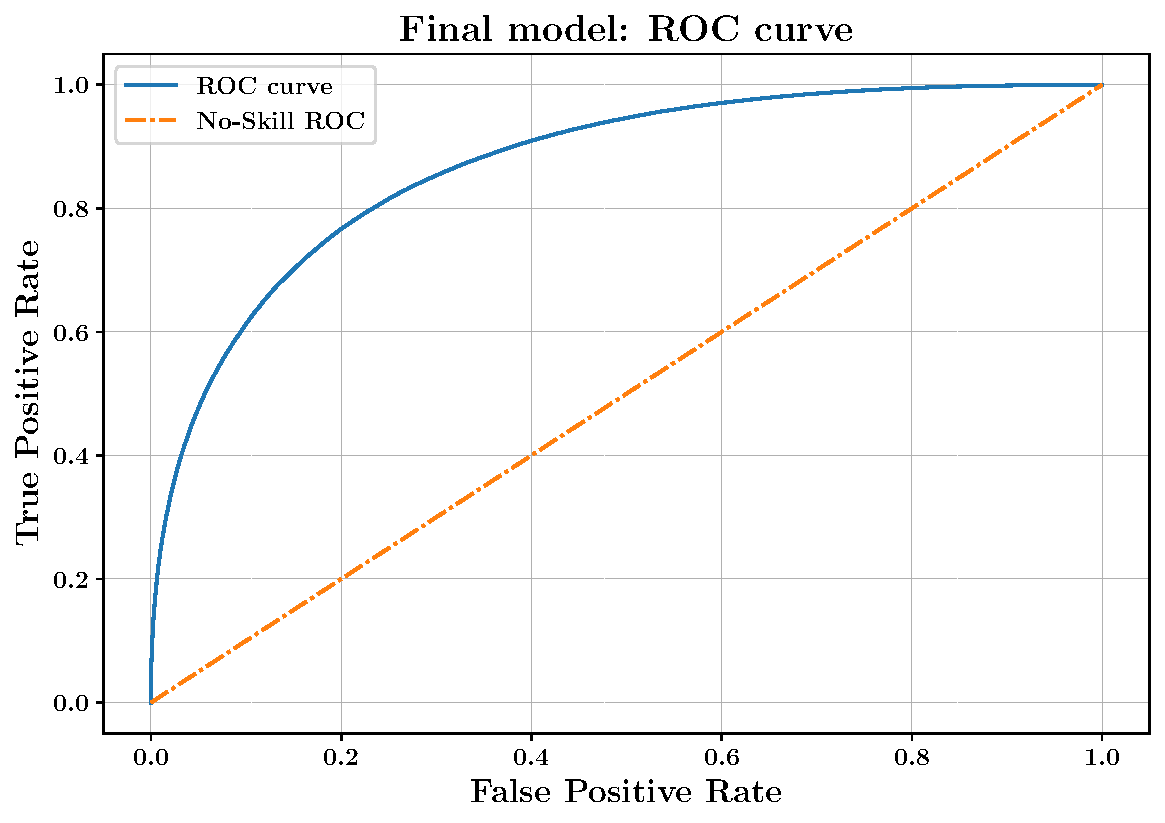
\includegraphics[height=5.8cm]{images/results/final/results_final_roc.pdf}
            \label{fig:results_final_roc}
        }
    \end{minipage}%
    \begin{minipage}[c]{0.50\linewidth}
        \vspace{0pt}
        \centering
        \subfloat[Final model confusion matrix]{
            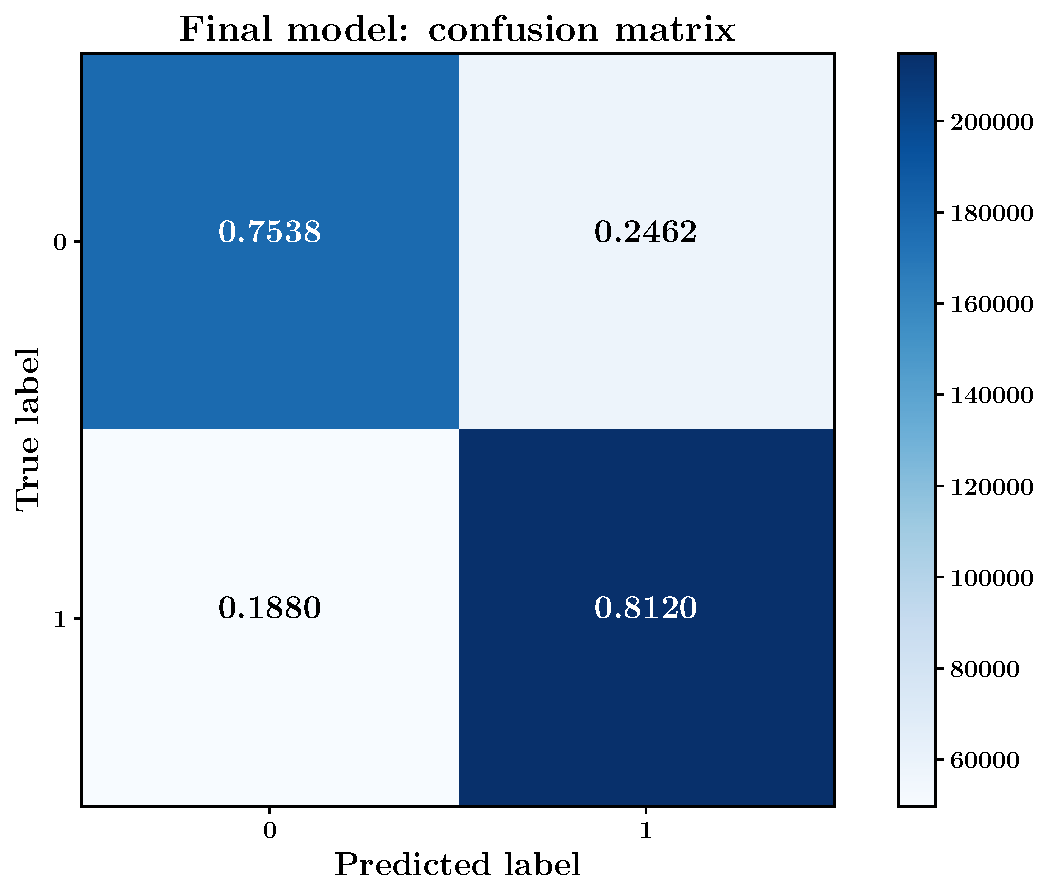
\includegraphics[height=5.8cm]{images/results/final/results_final_cm.pdf}
            \label{fig:results_final_cf}
        }
    \end{minipage}%
    \caption{Final TTN classifier predictions on test set. In \textbf{\ref{fig:results_final_roc}}, the ROC curve of the model prediction is showed, in \textbf{\ref{fig:results_final_cf}} the confusion matrix of the predicted classes is visualised. In particular, in the ladder the colormap represents the number of samples belonging to a certain prediction class.}
    \label{fig:results_final}
\end{figure*}


From this analysis we can extrapolate the final test accuracy and AUC:
\begin{align}
    \begin{aligned}
        \mathrm{Accuracy}_{\mathrm{final}} &= 78.46 \%   \\
        \mathrm{AUC}_{\mathrm{final}} &= 0.8694
    \end{aligned}
    \quad .
\end{align}
The ladder is below the best result obtained by \cite{baldi}, namely an AUC value of \( 0.885 \). However, the model trained in \cite{baldi} derives from a different approach and from a larger number of training epochs. Moreover, several improvements on the TTN best model are possible, such as a finer tuning of other hyperparameters and higher training epochs, but they go beyond the purpose of this work. These possibilities will be explored and tested for future work.

\end{document}